% Ch5.tex

\chapter{Multiple-instance multiple-label learning for the classification of frog calls with acoustic event detection}
\label{cha:cha6MIML}


\section{Introduction}
\label{sec:intro}

This chapter presents a method for the classification of simultaneously vocalising frog species in low SNR recordings. In chapter 4 and 5, frog call classification is solved using a SISL framework, which cannot reflect the nature of the low SNR recordings. Most low SNR recordings often 
consist of multiple simultaneously animal vocal activities including frogs, birds, crickets and so on. This character of low SNR recordings makes the multiple-instance multiple-label (MIML) learning a suitable classification framework for addressing. 
To be specific, individual frog syllables in one audio clip is regarded as \textit{multiple instance}, and the frog species included in that audio clip denotes \textit{multiple labels}. 
The key part of this MIML classification framework for frog calls is to detect individual syllables. After syllables detection, standard acoustic features and MIML classifiers can then be used to perform the MIML classification.


To evaluate our proposed classification framework, a representative sample of 342 10-seconds recordings was exported from the database and split into testing and training sets. The performance is evaluated based on the MIML learning measures. Experimental results demonstrate the MIML classification framework can be adopt to classify multiple simultaneously vocalising frog species in low SNR recordings.






\section{Conference paper - Multiple-instance multiple-label learning for the classification of frog calls with acoustic event detection}

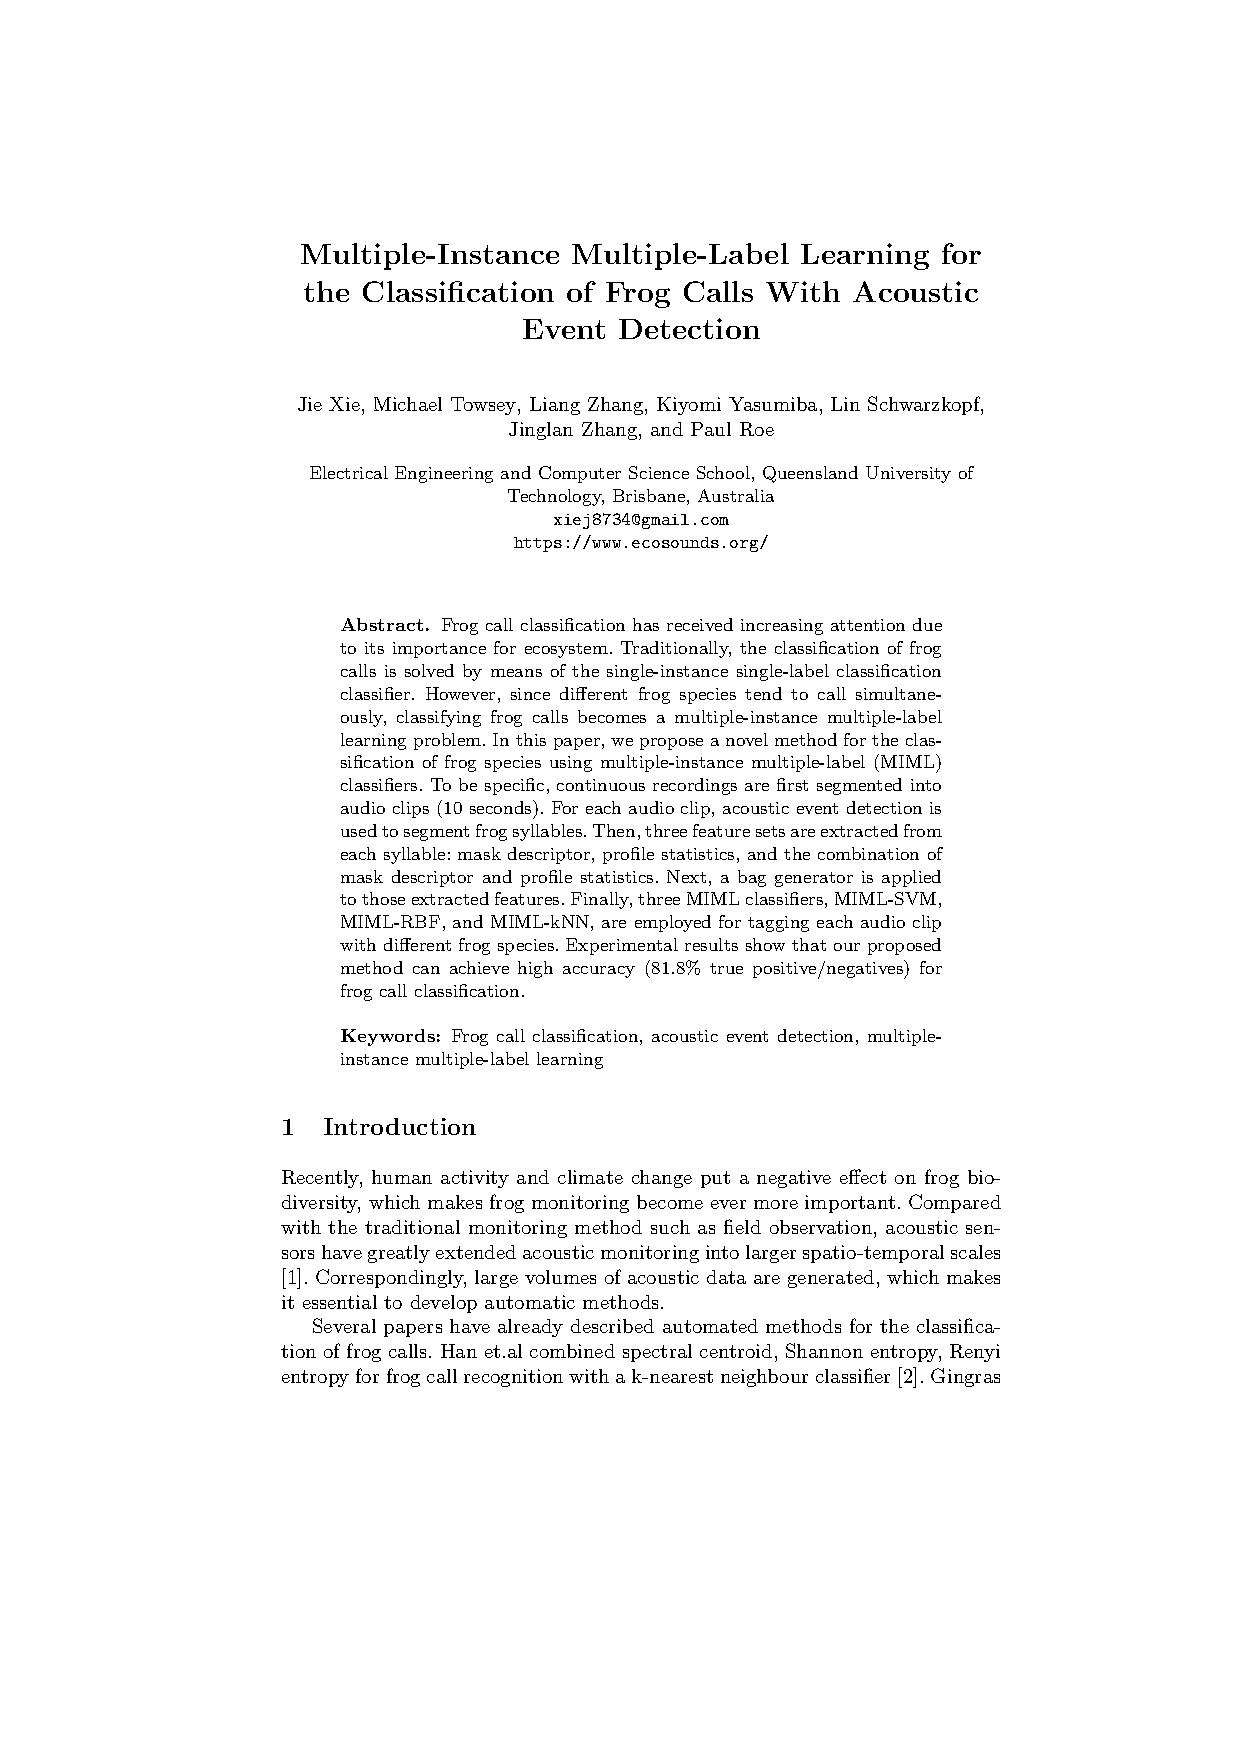
\includepdf[pages=-, pagecommand={},width=1.5\textwidth]{Ch6_paper.pdf}

